% !TEX TS-program = pdflatex
% !TEX encoding = UTF-8 Unicode

% This is a simple template for a LaTeX document using the "article" class.
% See "book", "report", "letter" for other types of document.

\documentclass[11pt]{article} % use larger type; default would be 10pt

\usepackage[utf8]{inputenc} % set input encoding (not needed with XeLaTeX)

%%% Examples of Article customizations
% These packages are optional, depending whether you want the features they provide.
% See the LaTeX Companion or other references for full information.

%%% PAGE DIMENSIONS
\usepackage{geometry} % to change the page dimensions
\geometry{a4paper} % or letterpaper (US) or a5paper or....
% \geometry{margin=2in} % for example, change the margins to 2 inches all round
% \geometry{landscape} % set up the page for landscape
%   read geometry.pdf for detailed page layout information

\usepackage{graphicx} % support the \includegraphics command and options

% \usepackage[parfill]{parskip} % Activate to begin paragraphs with an empty line rather than an indent

%%% PACKAGES
\usepackage{booktabs} % for much better looking tables
\usepackage{array} % for better arrays (eg matrices) in maths
\usepackage{paralist} % very flexible & customisable lists (eg. enumerate/itemize, etc.)
\usepackage{verbatim} % adds environment for commenting out blocks of text & for better verbatim
\usepackage{subfig} % make it possible to include more than one captioned figure/table in a single float
% These packages are all incorporated in the memoir class to one degree or another...

%%% HEADERS & FOOTERS
\usepackage{fancyhdr} % This should be set AFTER setting up the page geometry
\pagestyle{fancy} % options: empty , plain , fancy
\renewcommand{\headrulewidth}{0pt} % customise the layout...
\lhead{}\chead{}\rhead{}
\lfoot{}\cfoot{\thepage}\rfoot{}

%%% SECTION TITLE APPEARANCE
\usepackage{sectsty}
\allsectionsfont{\sffamily\mdseries\upshape} % (See the fntguide.pdf for font help)
% (This matches ConTeXt defaults)

%%% ToC (table of contents) APPEARANCE
\usepackage[nottoc,notlof,notlot]{tocbibind} % Put the bibliography in the ToC
\usepackage[titles,subfigure]{tocloft} % Alter the style of the Table of Contents
\usepackage{graphicx}
\graphicspath{ {image/} }

\usepackage{algorithm}
\usepackage{amsmath}

\renewcommand{\cftsecfont}{\rmfamily\mdseries\upshape}
\renewcommand{\cftsecpagefont}{\rmfamily\mdseries\upshape} % No bold!

%%% END Article customizations

%%% The "real" document content comes below...

\title{CS770: Assignment 1}
\author{Ronghao Yang\\20511820}
%\date{} % Activate to display a given date or no date (if empty),
         % otherwise the current date is printed 

\begin{document}
\maketitle

\section{Question 1}
For $f(x)$, I select \begin{equation}f(x) = (x^{2}+x)sin(x)^{2}\end{equation}\begin{equation}f(x)^{'}=(2x+1)sin(x)^{2}+(x^{2}+x)sin(2x)\end{equation}\begin{equation}f(x)^{''} = 2sin(x)^{2}+2(2x+1)sin(2x)+2(x^{2}+x)cos(2x)\end{equation} As for my chosen point, I set $x$ to be 2.

\subsection{Question 1.a}
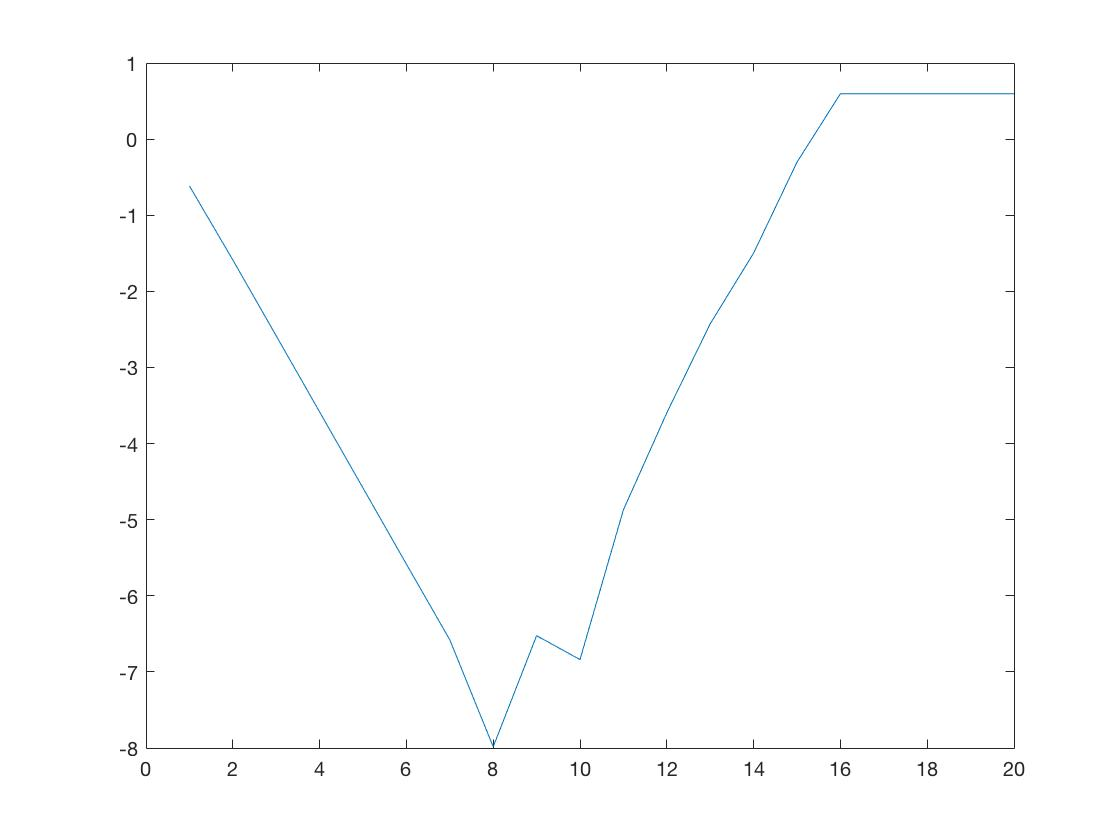
\includegraphics[scale=0.4]{q11.jpg}

\subsection{Question 1.b}
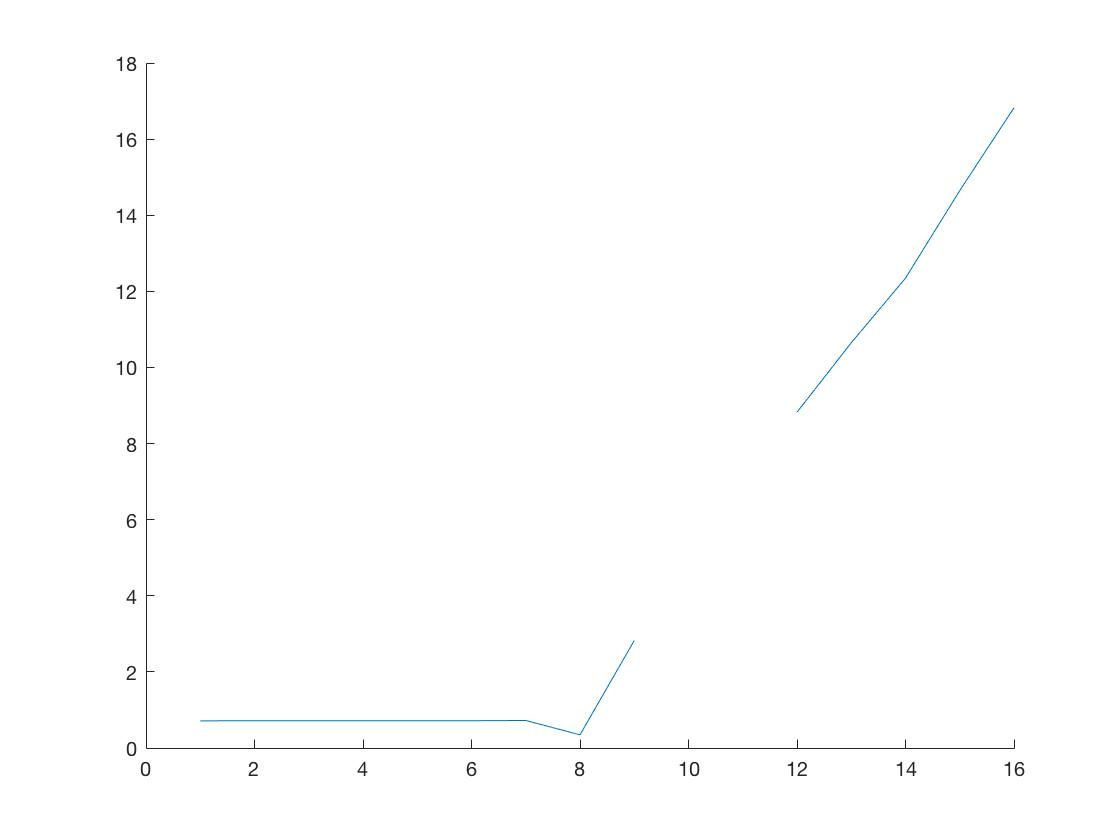
\includegraphics[scale=0.4]{q12.jpg}\\
The missing part in the graph is -Inf, this is from the errors being 0(therefore $log10(error) = -Inf$) when $h$ has the value of $10^{10}$ and $10^{11}$

\section{Question 2}
\textbf{Inexactness of algebraic operations}:\\
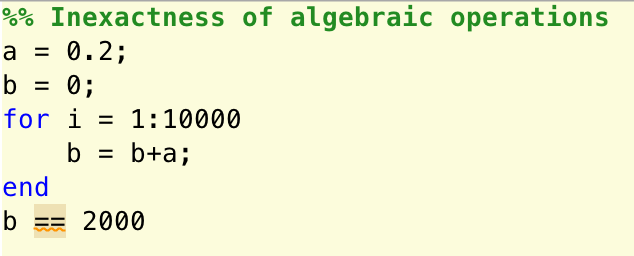
\includegraphics{q21}\\
b is supposed to be 2000, however, due to the error generated in floating point operations, $b==2000$ is evaluated to false. \\\\
\textbf{Non-commutativity of algebraic operations}:\\
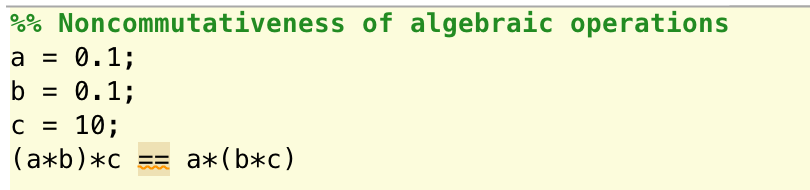
\includegraphics{q22}\\
(a*b)*c is supposed to be equal to a*(b*c), however, due to the error generated in floating point operations, $(a*b)*c == a*(b*c)$ is evaluated to false. \\\\
\textbf{Cancellation of errors}:\\
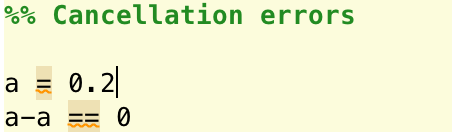
\includegraphics{q23}\\
Although $a = 0.2$ is a approximated, it's error is cancelled when $a-a$ is performed, therefore, $a-a == 0$ is evaluated to true. 
\section{Question 3}
Computation by $Matlab$, the two roots are:
\begin{equation}x_{1} = 9.999999999999999e+07\end{equation}
\begin{equation}x_{1} = 1.000000000000000e-08\end{equation}
However, computation by a hand calculator gives:
\begin{equation}x_{1} = 10^{8}\end{equation}
\begin{equation}x_{1} = 0\end{equation}

\section{Question 4}
\subsection{Question 3.1}
1) Signs and modulus:\\
Since we have 1 bit for sign, we have 31 bits for representing the magnitude of a number. Therefore, there are $2^{31}$ different magnitudes can be represented, and by adding the sign, we have $2\times2^{31}-1 = 2^{32}-1$ different numbers can be represented.(If +0 and -0 are counted as two different numbers, then there are $2^{32}$ different numbers) \\
2) 2's complement:\\ 
When using 2's complement for representing numbers, we could have representations for $2^{32}$ different numbers. \\\\
2's complement is the representation for zero unique.
\subsection{Question 3.2}
When using unsigned numbers, numbers range from $0$ to $2^{16}-1$($0$ to $65535$ in decimal).\\
When using signed numbers, numbers range from $-2^{15}$ to $2^{15}-1$ ($-32768$ to $32767$ in decimal).

\subsection{Question 3.3}
1: 00000001\\
10: 00001010\\
100: 01100100\\
-1: 11111111\\
-10: 11110110\\
-100: 10011100\\\\
For example, $100 + (-100)$, which in binary representation is $01100100+10011100 = 100000000$, since it uses 8 bits for number representation, the first bit $1$ is discarded, this gives us 0.
\subsection{Question 3.4}
With 32 bits representation, a negative number $-x$ is represented using $2^{32}-x$, since -x is negative, -x ranges from $-2^{31}$ to $-1$, then x ranges from $1$ to $2^{31}$, then $2^{32}-x$ ranges from $2^{31}$ to $2^{32}-1$, this always leaves the first bit of the 32 bits 1. Therefore, all the negative numbers have leading bit 1.\\
Similarly, for a positive x, x ranges from $0$ to $2^{31}-1$, this always leaves the first bit of the 32 bits 0. Therefore, all the positive numbers have leading bit 0.
\subsection{Question 3.5}
The last step to complete the process is add 1 to it. Let's say we have 32 bits, $x$ is a positive number, if we simply flip the bits without adding a 1 at the end, $x + (-x) = 2^{32}-1$. By definition $-x = 2^{32}-x$, therefore, we should add 1 after we flip the bits.
\subsection{Question 3.6}
In binary representation, 50,-50,100,-100 are represented in the following:\\
50: 00110010\\
-50: 11001110\\
100: 01100100\\
-100: 10011100\\\\
1) $50$+ ($-100$) = 00110010 + 10011100 =  11001110 which is -50 in decimal.\\
2) $100$+ ($-50$) = 01100100 + 11001110 = 100110010, since the first digit is discarded, the answer is 00110010, which is 50 in decimal.\\
3) $50$ + $50$ = 00110010 +  00110010 = 01100100, which is 100 decimal, no overflow occurred.





\end{document}
